\documentclass[a4paper,11pt]{report}
\usepackage[spanish,mexico]{babel}
\usepackage[utf8]{inputenc}
\usepackage[T1]{fontenc}
\usepackage{amsmath}
\usepackage{amssymb}
\usepackage{wasysym}
\usepackage[dvipsnames,pdftex]{color}
\usepackage[colorinlistoftodos]{todonotes}
%\usepackage{helvet}
%\renewcommand{\familydefault}{\sfdefault}
\setlength{\oddsidemargin}{0in}
\usepackage{here}
\usepackage{geometry}
 \setlength{\textwidth}{6.4in}
 \setlength{\topmargin}{0in}
 \setlength{\voffset}{-0.6in}
 \setlength{\hoffset}{-0.2in}
 \setlength{\textheight}{9.7in}
 \setlength{\topskip}{0in}
 \setlength{\parskip}{2ex}
 \renewcommand{\baselinestretch}{1.5}
\usepackage{diagbox}
\usepackage{array}
\usepackage{listings}
\usepackage{caption}
%%% comandos definidos por el usuario
\begin{document}
\setcounter{page}{1}
\pagenumbering{roman}
\thispagestyle{empty}
\begin{center}
{\huge UNIVERSIDAD NACIONAL DE INGENIERÍA}\\[0.9cm]
{\Large FACULTAD DE INGENIERÍA MECÁNICA}\\[0.6in]
\end{center}
\begin{figure}[h]
\begin{center}

\includegraphics[scale=0.33]{logoUNI.png}
\vspace{0cm}
\end{center}
\end{figure}
\vspace{0.5cm}
\begin{center}
INFORME DE LABORATORIO\\
LABORATORIO DE INGENIERÍA MECÁNICA\\[14mm]
{\large MEDICIÓN DE TEMPERATURA}\\[10mm]
\vfill
LIMA - PERÚ \hfill SEPTIEMBRE 2019
\end{center}
\newpage
\thispagestyle{empty}
\begin{center}
{\Huge MEDICIÓN DE TEMPERATURA}\\[0.7cm]
\small ENTREGADO:\\[0.3cm]
\small 15 SEPTIEMBRE 2019\\[2.9cm]
\end{center}
\begin{flushleft}
{\large ALUMNOS:}\\[2cm]
\end{flushleft}
\begin{tabular}{c@{\hspace{0.5in}}c}
\rule[1pt]{2.6in}{1pt}&\rule[1pt]{2.6in}{1pt}\\
Carranza Zavala David, 20174065E & Huaroto Villavicencio Josue, 20174070I\\[2.5cm]
\rule[1pt]{2.6in}{1pt}&\rule[1pt]{2.6in}{1pt}\\
Landeo Sosa Bruno, 20172024J & Lino Carbajal Franklin, 20110146D\\[2.5cm]
\rule[1pt]{2.6in}{1pt}&\rule[1pt]{2.6in}{1pt}\\
Quesquen Vitor Angel, 20170270C & Sotelo Cavero Sergio, 20172125K\\[2.5cm]
\end{tabular}
%\begin{center}
%\begin{tabular}{c@{\hspace{0.5in}}c}
%\rule[1pt]{3.14in}{1pt}\\
%Sotelo Cavero Sergio, 20172125K% & Nombre 5, 2017 \\[1.5cm]
%\end{tabular}
%\end{center}
%\begin{center}
%\begin{tabular}{c@{\hspace{0.6in}}c}
%\rule[1pt]{3.14in}{1pt}\\
%Huaroto Villavicencio Josué, 20174070I \\[2.5cm]
%\rule[1pt]{3.14in}{1pt}\\
%Landeo Sosa Bruno, 20172024J \\[2.5cm]
%\rule[1pt]{3.14in}{1pt}\\
%Quesquen Vitor Angel, 2017 \\[2.5cm]
%\rule[1pt]{3.14in}{1pt}\\
%Sotelo Cavero Sergio, 20172125K
%\end{tabular}
%\end{center}
%\begin{center}
%\begin{tabular}{c}
%\rule[1pt]{3.14in}{1pt}\\
%Huaroto Villavicencio Josué, 20174070I \\[2.5cm]
%\end{tabular}
%\end{center}

%\rule[1pt]{3.14in}{1pt}\\
%Maguiña Amaya Wladimir, 20172019F \\[3cm]
%\rule[1pt]{3.14in}{1pt}\\
%Luis Sosa Jose, 19774147I \\[3cm]
%\rule[1pt]{3.14in}{1pt}\\
%Sotelo Cavero Sergio, 20172125K
%\end{tabular}
%\end{center}
%\\[0.7cm]
{\large PROFESOR:} \\[0.6cm]
\begin{center}
\begin{tabular}{c}
\rule[3pt]{4.8in}{1pt}\\[1pt]
ING. MORALES TAQUIRI OSWALDO
\end{tabular}
\end{center}
\vfill
%\newpage
%\begin{center}
%{\Large \bf{RESUMEN}}
%\end{center}
\newpage
\tableofcontents
%\listoffigures
%\addcontentsline{toc}{chapter}{Índice de figuras}
\newpage
\pagenumbering{arabic} %%% esto es para regresar el modo de numeración a numeración arábiga
\setcounter{page}{1}  %%% empezamos en página 1
%\part{Introducción}
\chapter{Objetivos}
\begin{enumerate}
\item Aprender ciertas técnicas de medición para maximizar la exactitud aunque se utilicen instrumentos no tan precisos.
\item Adquirir experiencia en la tabulación de temperaturas para aplicarlas en el campo laboral.
\item Comprender como funciona cada instrumento de medición de la temperatura.
\item Comparar las lecturas de todos los instrumentos y ver que tanto error presentan comparado con el instrumento base.
\end{enumerate}
\chapter{Marco teórico}
\section{Termómetro de inmersión parcial}
Un termómetro de inmersión parcial está diseñado para hacer lecturas de temperatura mediante la inmersión de una determinada longitud de forma vertical, que va desde el bulbo hasta una marca que estará al mismo nivel del fluido, este tipo de instrumento es de gran ayuda para mediciones donde la profundidad del fluido sea poca, es decir se volverían obsoletos el termómetro de inmersión total y completa porque estas marcarían un valor erróneo al no poder sumergirse completamente en forma vertical; sin embargo no sería de mucha ayuda el de inmersión parcial o cualquier otro termómetro de vidrio si no está calibrado en todo el rango de medición además depende de que tanto se ha dilatado el tubo capilar y otros factores más.\\
A continuación, se mostrará una comparación entre los 3 termómetros de vidrio.
\begin{figure}[H]
\begin{center}
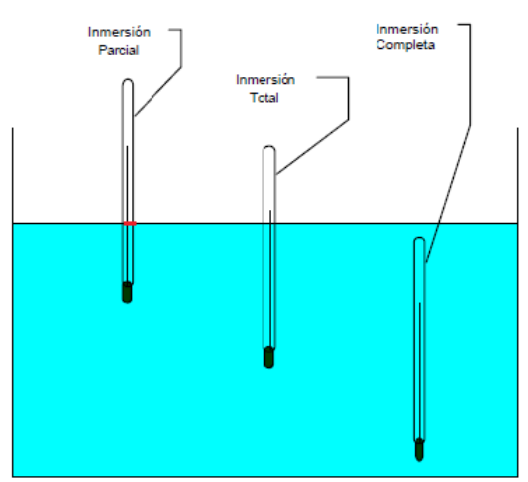
\includegraphics[scale=0.4]{parcial1.png}
\end{center}
\end{figure}
\section{Termómetro de inmersión total}
Los termómetros de vidrio son instrumentos precisos y económicos que miden las temperaturas de los liquidos o gases. Los termometros de vidrio cumplen con la Escala de Temperatura Internacional de 1990(ITS-90). Los termometros ASTM varian de 5.5 a 8 mm en diámetro.\\
\textbf{Características.} Soporta temperaturas de -10$^{\circ}$C hasta 150$^{\circ}$C.\\
\textbf{Exactitud.} La exactitud de un termometro de vidrio tipico es de aproximadamente $\pm$1 division de la escala.\\
\textbf{Usos.} Diseñado para medir la temperatura de diferentes sustancias.\\
\textbf{Especificaciones.}
\begin{itemize}
\item Resistente a muy altas temperaturas.
\item Mide la temperatura de cualquier clase de liquidos que se encuentren en exposicion ambiental o en reaccion quimica.
\item Debido al material del que está hecho es necesario tener cuidado, pues es muy frágil y se rompe con facilidad.
\end{itemize}
\subsection{Correcciones del cuerpo emergente}
Evite las mediciones incorrectas cuando un termometro de inmersion total no se puede surmergir correctamente. Determine la correccion del cuerpo aproximada con estas formulas:
\begin{itemize}
\item \textbf{Para termómetros de mercurio en Fahrenheit.} $ = 9\cdot 10^{-5} \cdot n \cdot (T-t) ^{\circ} F$
\item \textbf{Para termómetros de mercurio en Celsius.} $ = 16\cdot 10^{-5} \cdot n \cdot (T-t) ^{\circ} C$
\item \textbf{Para termómetros rellenos de alcohol en Fahrenheit.} $ = 6\cdot 10^{-5} \cdot n \cdot (T-t) ^{\circ} F$
\item \textbf{Para termómetros rellenos de alcohol en Celsius.} $ = 1\cdot 10^{-3} \cdot n \cdot (T-t) ^{\circ} C$
\end{itemize}
Donde $T$ es la temperatura del baño (la temperatura indicada en el termometro), $t$ es la temperatura promedio de la parte emergente del cuerpo y $n$ es la cantidad de grados del termometro emergente. Para determinar $t$, sostenga un termómetro auxiliar junto a la parte emergente del cuerpo.
\section{Termocuplas}
Las termocuplas son el sensor de temperatura más común utilizado industrialmente.
Una termocupla se hace con dos alambres de distinto material unidos en un extremo (soldados generalmente). Al aplicar temperatura en la unión de los metales se genera un voltaje muy pequeño (efecto Seebeck) del orden de los milivolts el cual aumenta con la temperatura. Por ejemplo, una termocupla ``tipo J'' está hecha con un alambre de hierro y otro de constantán (aleación de cobre y nickel) Al colocar la unión de estos metales a 750$^{\circ}$C, debe aparecer en los extremos 42.2 milivolts.
\begin{figure}[H]
\begin{center}
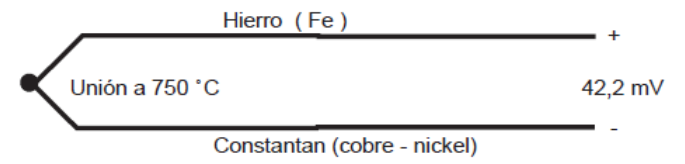
\includegraphics[scale=0.5]{termocupla1.png}
\end{center}
\end{figure}
Normalmente las termocuplas industriales se consiguen encapsuladas dentro de un tubo de acero inoxidable u otro material, en un extremo está la unión y en el otro el terminal eléctrico de los cables, protegido adentro de una caja redonda de aluminio (cabezal).
\begin{figure}[H]
\begin{center}
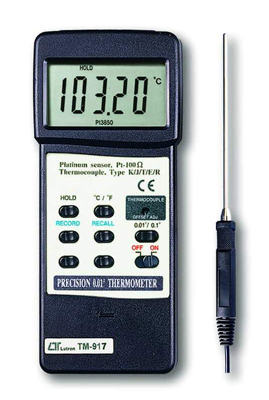
\includegraphics[scale=0.5]{termocupla2.jpg}
\end{center}
\end{figure}
\subsection{Tipos de termocuplas}
Existen una infinidad de tipos de termocuplas, en la tabla aparecen algunas de las más comunes, pero casi el 90\% de las termocuplas utilizadas són del tipo J o del tipo K.
\begin{center}
\begin{tabular}{|c|c|c|c|c|}
\hline 
Termocupla & Cable + Aleación & Cable - Aleación & Rango $^{\circ}$ C & Volts (mV) \\ 
\hline 
J & Hierro & Cobre/Nickel & (-180,750) & 42.2 \\ 
\hline 
K & Nickel/Cromo & Nickel/Aluminio & (-180,1372) & 54.8 \\ 
\hline 
T & Cobre & Cobre/Nickel & (-250,400) & 20.8 \\ 
\hline 
R & 87\% Platino + 13\% Rhodio & Platino & (0,1767) & 21.09 \\ 
\hline 
S & 90\% Platino + 10\% Rhodio & Platino & (0,1767) & 18.68 \\ 
\hline 
B & 70\% Platino + 30\% Rhodio & 94\% Platino + 6\% Rhodio & (0,1820) & 13.814 \\ 
\hline 
\end{tabular} 
\end{center}
\subsection{Usos típicos en la industria}
Las termocuplas tipo J se usan principalmente en la industria del plástico, goma y fundición de metales a bajas temperaturas (Zamac, Aluminio). La termocupla K se usa típicamente en fundición y hornos a temperaturas menores de 1300$^{\circ}$C, por ejemplo fundición de cobre y hornos de tratamientos térmicos. Las termocuplas R, S, B se usan casi exclusivamente en la industria siderúrgica (fundición de acero).
\subsection{Linealización}
La dependencia entre el voltaje entregado por la termocupla y la temperatura no es lineal (no es una recta), es deber del instrumento electrónico destinado a mostrar la lectura, efectuar la linealización, es decir tomar el voltaje y conociendo el tipo de termocupla, ver en tablas internas a que temperatura corresponde este voltaje.
\section{Termómetro bimetálico}
Una termómetro bimetálico está constituida por dos láminas de metal, cada una de ellas con diferente coeficiente de dilatación, superpuestas y soldadas entre sí. De este modo se consigue que cuando se calientan, al dilatarse cada una de ellas de forma distinta, el conjunto se deforma, pudiendo aprovecharse esta deformación para la apertura o cierre de un contacto eléctrico, cuya actuación dependería de la temperatura. Aplicaciones muy comunes de los contactos formados por láminas bimetálicas se encuentran en planchas, tostadores, estufas eléctricas y otros electrodomésticos que llevan un termostato, así como en elementos de protección eléctrica como los interruptores magnetotérmicos.
\begin{figure}[H]
\begin{center}
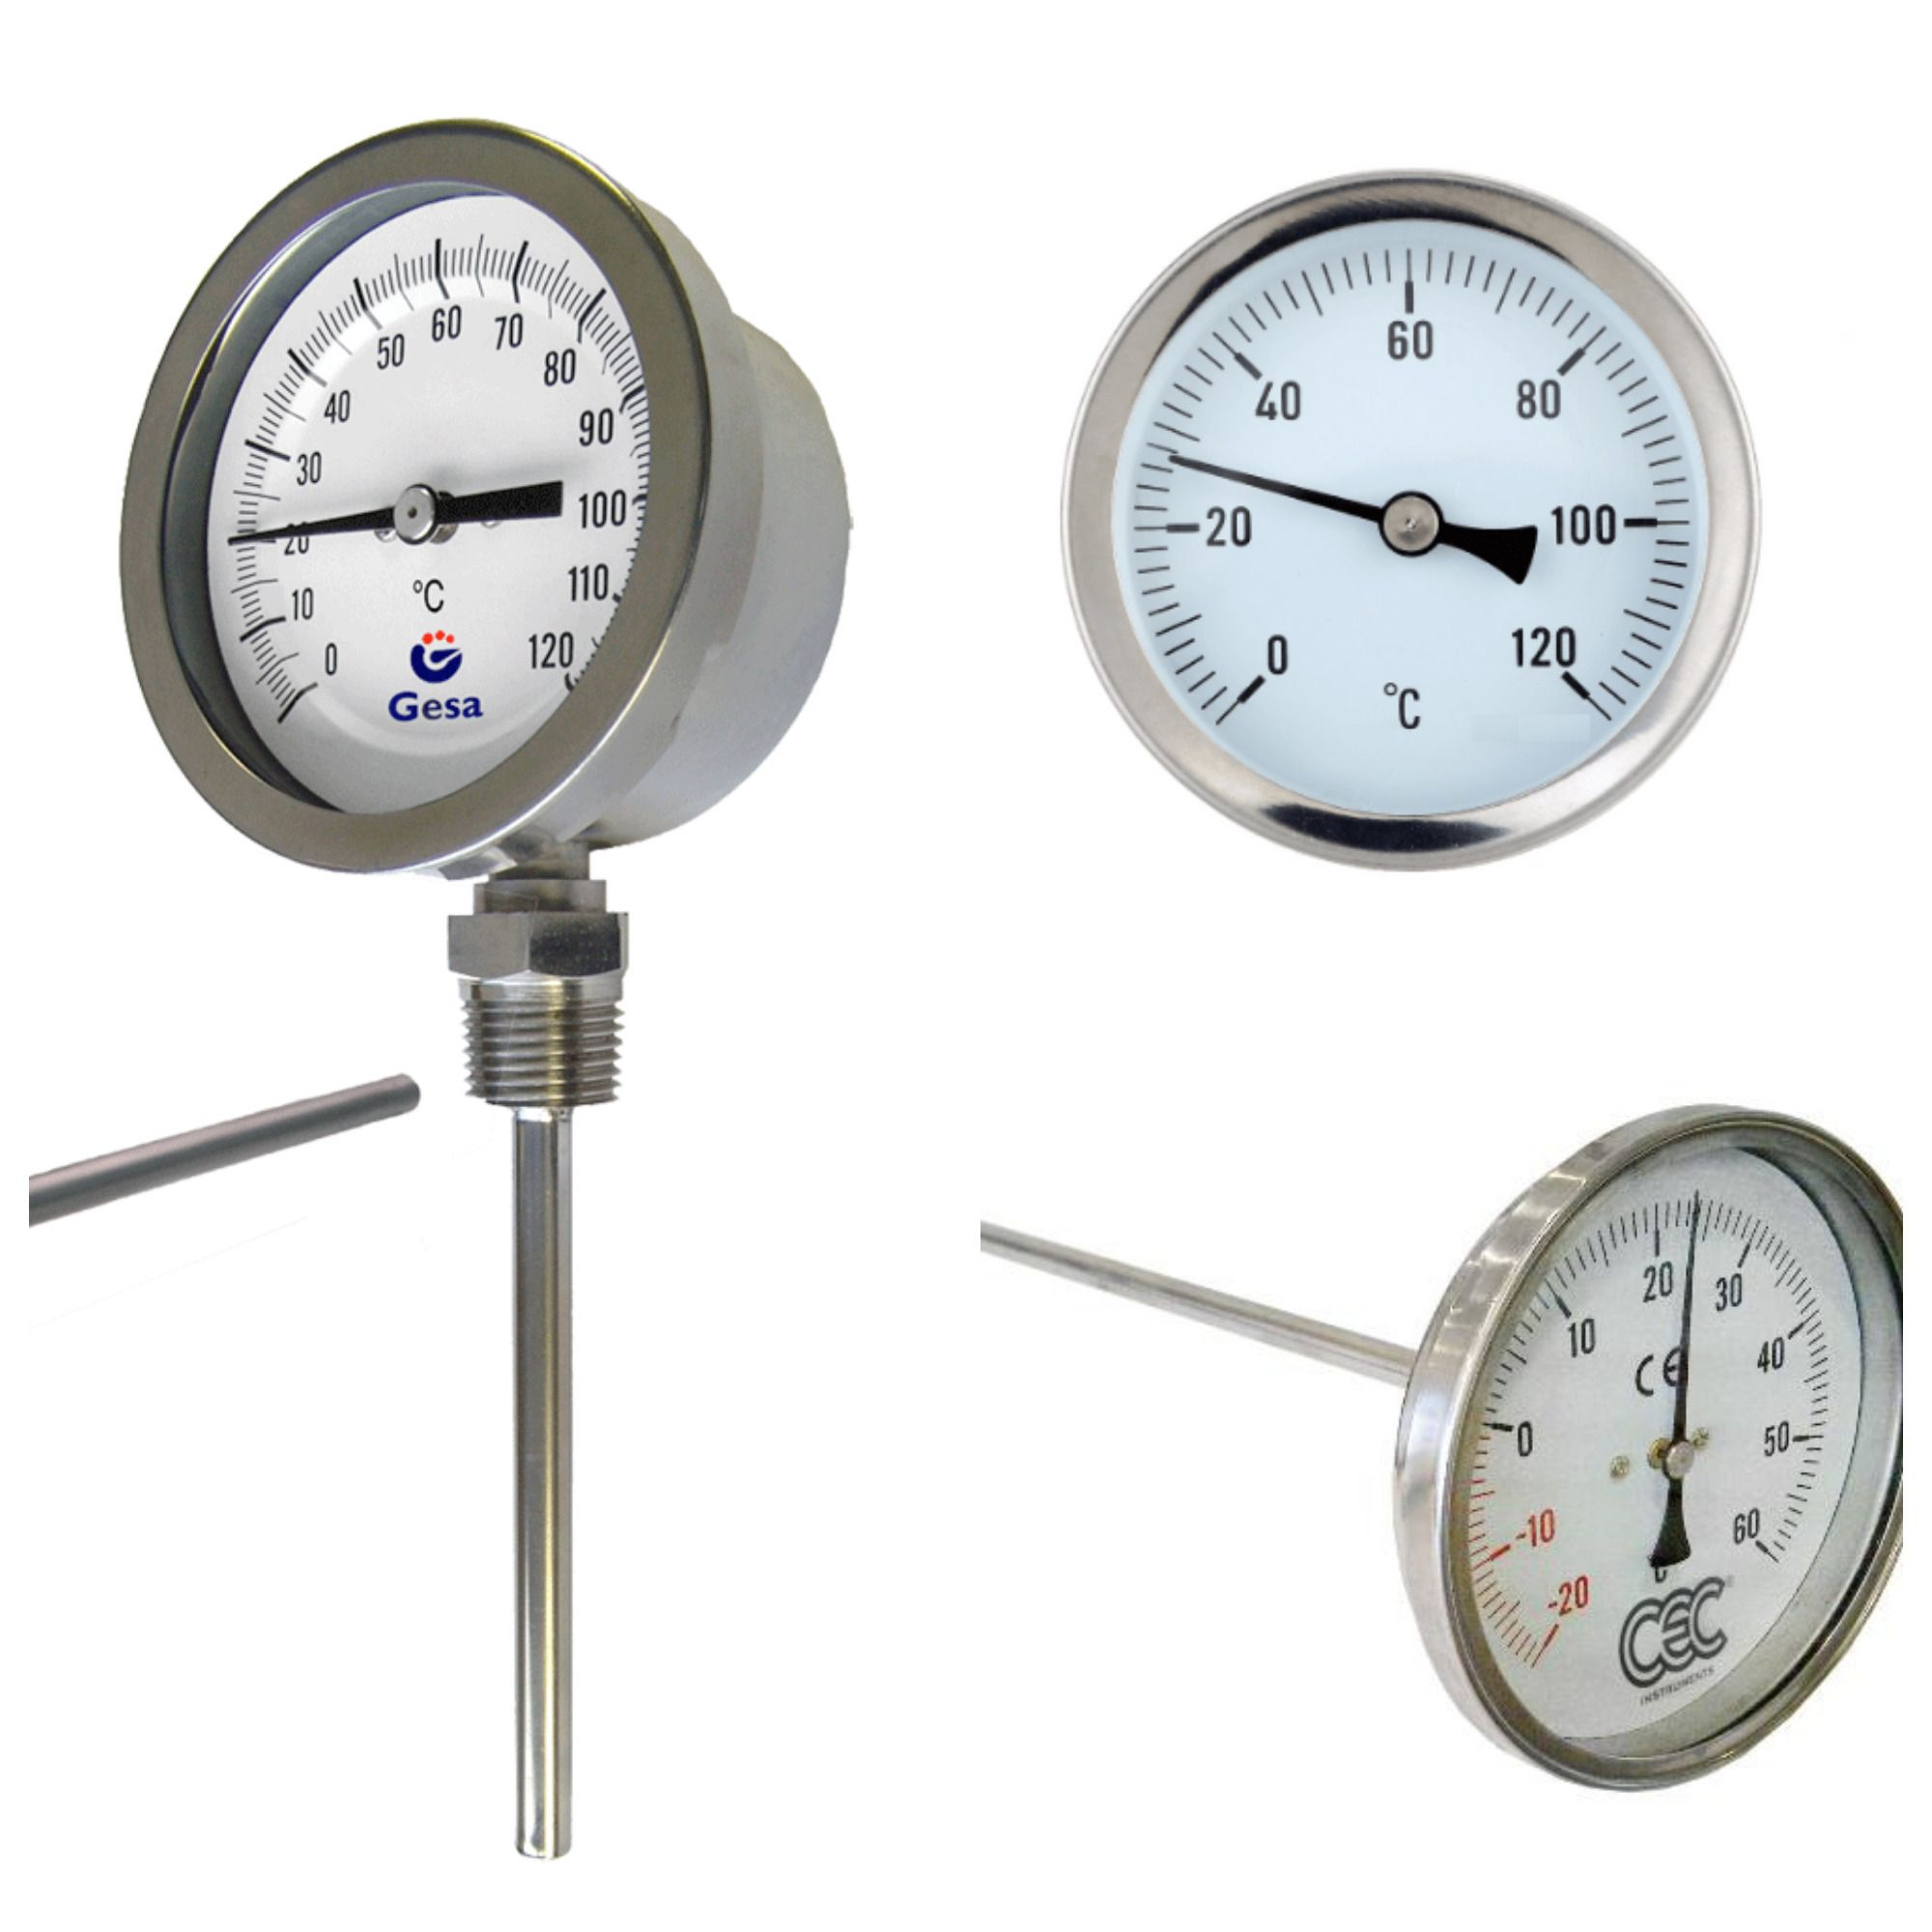
\includegraphics[scale=0.13]{bimetalico1.jpg}
\end{center}
\end{figure}
\chapter{Cálculos y resultados}
Para los gráficos se utilizó Python 3.7 en un entorno de jupyter notebook:
\begin{figure}[H]
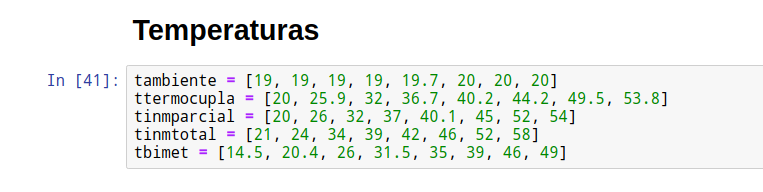
\includegraphics[scale=0.55]{Temperaturas.png}
\end{figure}
\section{Termocupla-Bimetálico}
\begin{figure}[H]
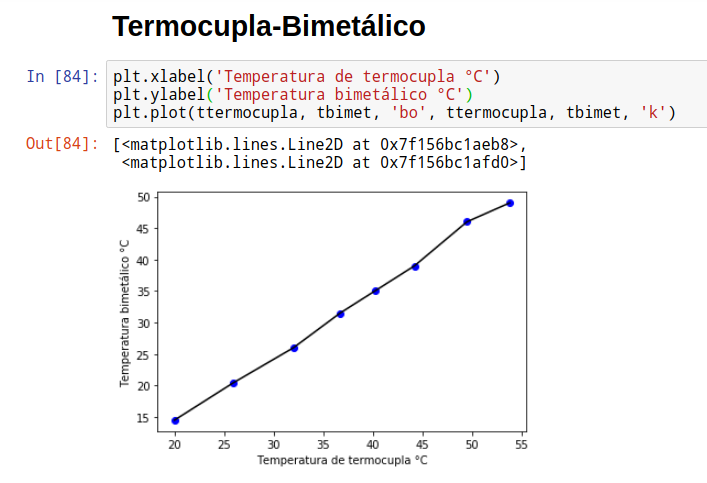
\includegraphics[scale=0.52]{pbimet1.png}
\end{figure}
\subsection{Error}
\begin{figure}[H]
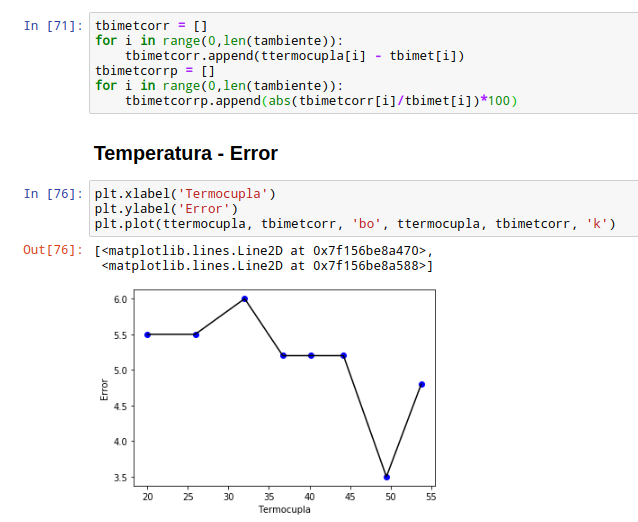
\includegraphics[scale=0.65]{pbimet2.png}
\end{figure}
\subsection{Error porcentual}
\begin{figure}[H]
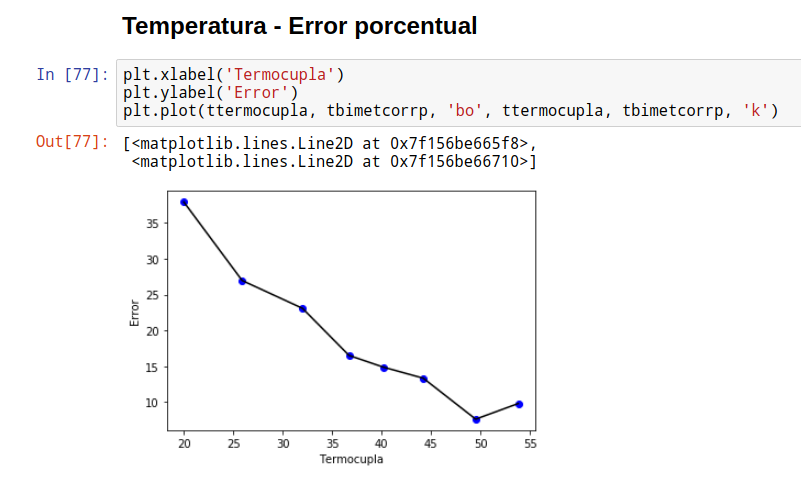
\includegraphics[scale=0.55]{pbimet3.png}
\end{figure}
\section{Termocupla-Total}
\begin{figure}[H]
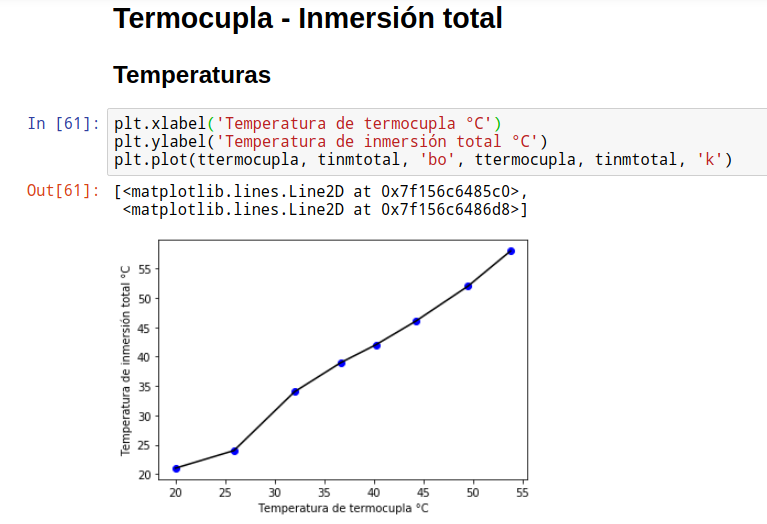
\includegraphics[scale=0.52]{ptotal1.png}
\end{figure}
\subsection{Error}
\begin{figure}[H]
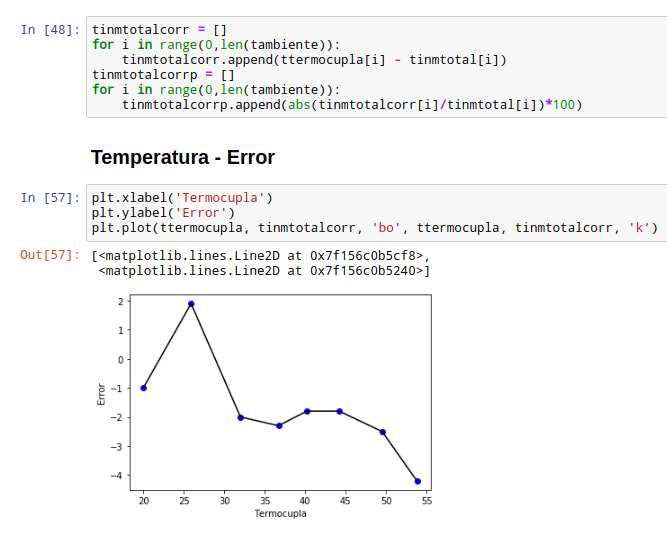
\includegraphics[scale=0.62]{ptotal2.png}
\end{figure}
\subsection{Error porcentual}
\begin{figure}[H]
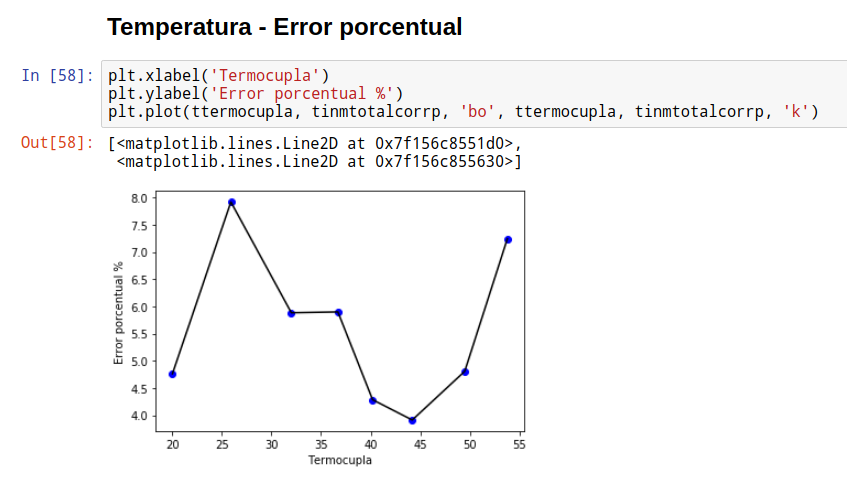
\includegraphics[scale=0.52]{ptotal3.png}
\end{figure}
\section{Termocupla-Parcial}
\begin{figure}[H]
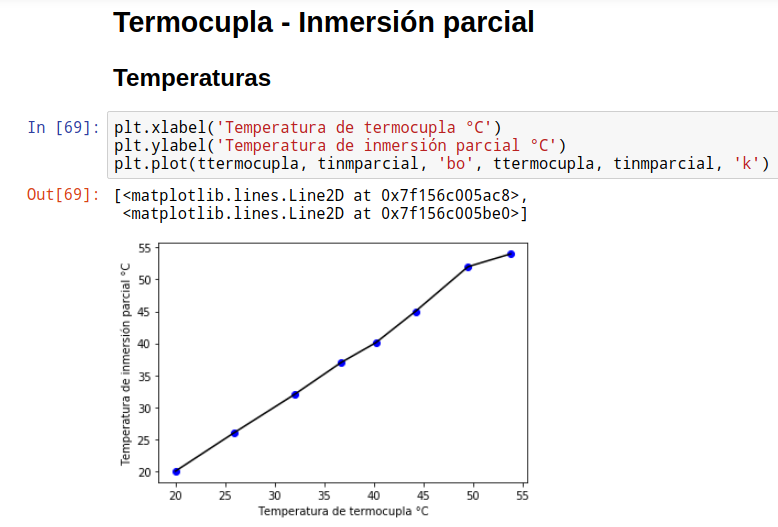
\includegraphics[scale=0.52]{pparcial1.png}
\end{figure}
\subsection{Error}
\begin{figure}[H]
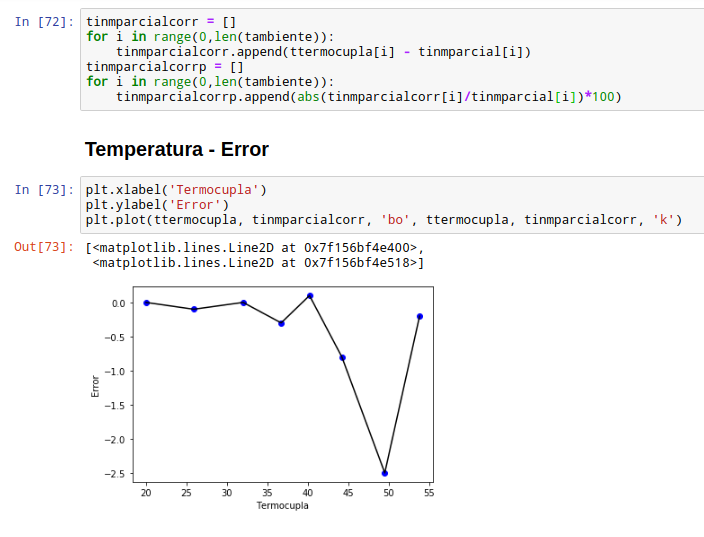
\includegraphics[scale=0.62]{pparcial2.png}
\end{figure}
\subsection{Error porcentual}
\begin{figure}[H]
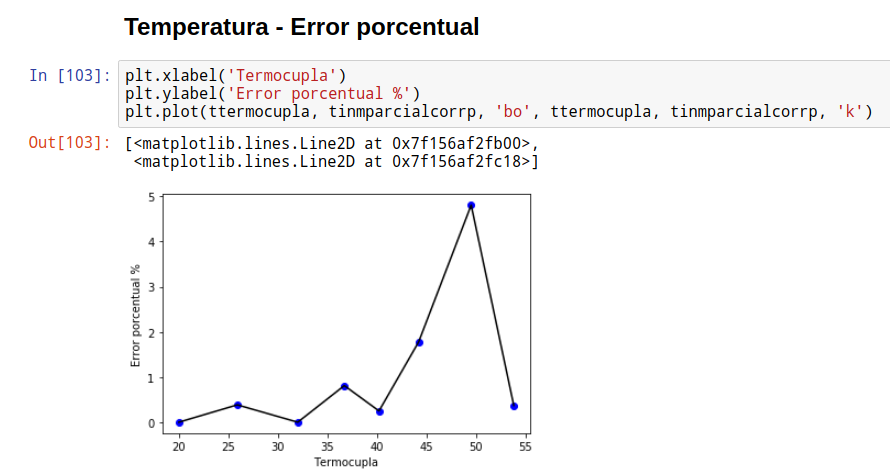
\includegraphics[scale=0.52]{pparcial3.png}
\end{figure}
\section{Errores cuadráticos medios}
\begin{figure}[H]
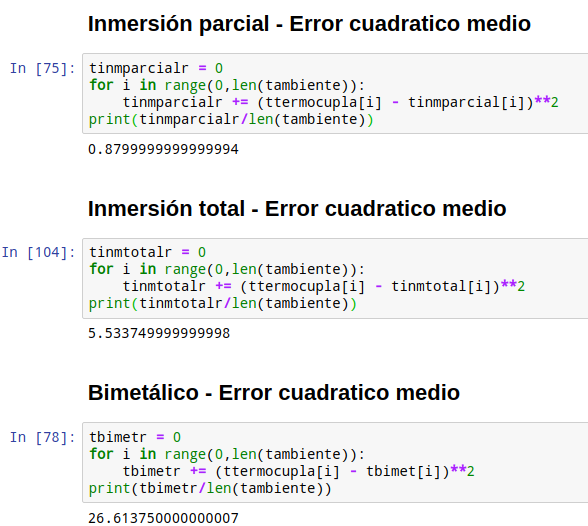
\includegraphics[scale=0.62]{cuadratico.png}
\end{figure}
%\part{Conclusiones y recomendaciones}
\chapter{Conclusiones}
\begin{enumerate}
\item El termómetro de inmersión parcial es el que mejores resultados ha obtenido.
\item El termómetro bimetálico dió errores muy grandes al comienzo. Dicho error fue disminuyendo conforme se hacía más mediciones, hasta llegar a menos de 10\% de error.
\item Precisar la ubicación del termómetro de inmersión total (ubicarlo completamente sumergido) ya que puede darnos una mala lectura.
\item Trabajar como temperatura patrón la termocupla de lectura digital porque es la que representa mayor sensibilidad, por ende tendrá mayor precisión. 
\item La tendencia de los instrumentos utilizados está muy asimilada a la realidad, es decir, el error es aceptable.
\item Cuando se apaga el calentador, se recomienda esperar hasta que la termocupla deje de aumentar de temperatura.
\end{enumerate}
\chapter*{Anexos}
\begin{figure}[H]
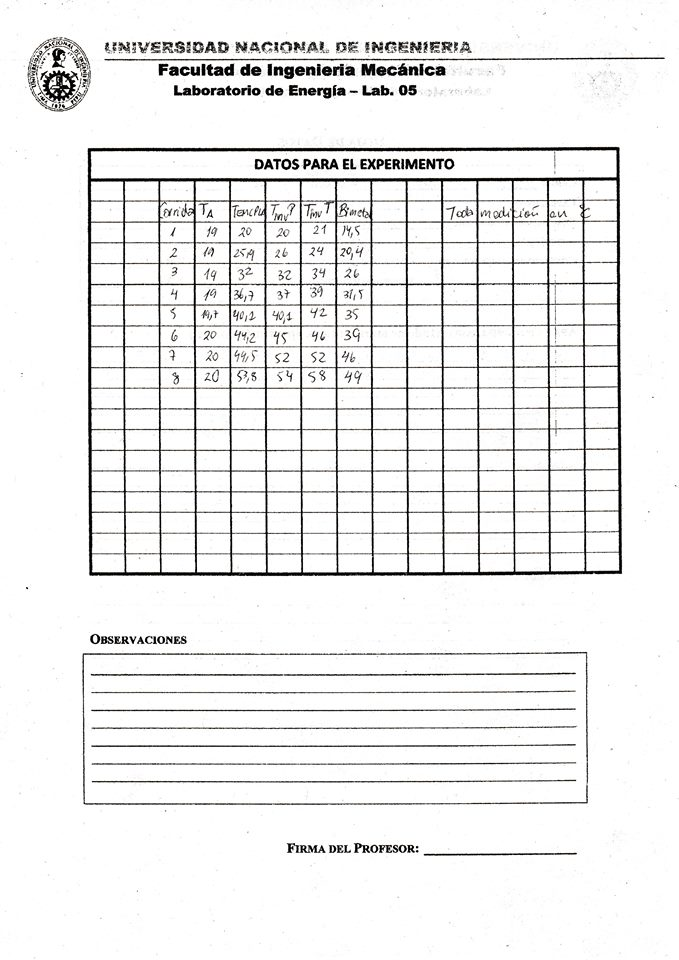
\includegraphics[scale=0.55]{datos.jpg}
\end{figure}
\begin{thebibliography}{99}  %%%este es un contador para el número de bibliografías utilizados.
\addcontentsline{toc}{chapter}{Bibliograf\'{\i}a} %%% Para introducir la bibliografía en el índice.
%\bibitem{Rahman}{Rahman,Aminur y Doe, Hidekazu; ``Ion transfer of tetraalkylammonium cations at an interface between 
%frozen aqueous solution and 1,2-dichloroethane".{\em{Journal of Electroanalytical Chemistry}} {\bfseries 424},159,(1997).}
\bibitem{Gro}{Casterona Machuca, J. (2019) ``El ingeniero industrial y el sistema de seguridad en las empresas''. }
%\bibitem{Gro}{Sadiku, Matthew N. ``Fundamemtos de circuitos eléctricos''. {\em{Mc Graw Hill}}}
%\bibitem{Ding}{Ding, Zhifeng. ``Spectroelectrochemistry and photoelectrochemistry of charge transfer at liquid/liquid
%interfaces". {\em {Tesis, EPFL,}}(1999).}
%\bibitem{AL}{Alonso, Jose M. \em{Técnicas de mecanizado 1}}
%\bibitem{AL}{Alonso, Jose M. ``Técnicas de mecanizado 1". {\em{Paraninfo}} {\bfseries España-Madrid}, 6-20, (2001).}
%\bibitem{Samec2}{Samec Z., Lhotsky A., Jänchenová H., y Marecek, V. ``Interfacial tension and impedance measurements
%of interfaces between two inmiscible electrolyte solutions". {\em{Journal of Electroanalytical Chemistry}} {\bfseries
%43}, 47, (2000).}
%\bibitem{Day}{Day R.A. y Underwood A.L. {\textit{Química Analítica Cuantitativa}},5ºed. Prentice-Hall, México, 1998. 45-48.}
%\bibitem{Keyser}{Farah Abud, Michel. ``Determinación de la vida útil en herramientales de corte endurecido por el proceso de borurización en pasta''. {\em{Instituto tecnológico y de estudios superiores de Monterrey}}}
%\bibitem{Zolotorevski}{Escalona, I. ``Máquinas: herramientas por arranque de viruta.''.{\em{El Cid Editor.}}}
%\bibitem{Lasheras}{Lasheras. ``Tecnología de los Materiales Industriales''.} 
%\bibitem{Dieter}{Dieter. ``Metalurgia mecánica''.}
%\bibitem{Apraiz}{Apraiz, J. ``Tratamiento Térmico de los Aceros''.}
%\bibitem{Smith}{Smith, William F. y Ph.D. Hashemi, Javad ``Ciencia e ingeniería de materiales". {\em{
%Madrid: McGraw-Hill, Interamericana de España.}} 570, (2004).} 
%\bibitem{Callister}{Callister, William D. y Rethwisch, David G. ``Introducción a la ingeniería de los materiales''. %{\em{Barcelona Reverté.}}, 960, (2007).} 
%\bibitem{Askeland}{Askeland, Donald R., Pradeep P. Phulé y Wright, Wendelin J. ``Ciencia e ingeniería de los materiales''.{\em{México, D.F. Internacional Thomson Editores.}} {\textit{$6^{ta}$ edición}}, 1004, (2012).}
%\bibitem{HARDBANDING}{Tabla de conversión de escala de durezas. \begin{verbatim}http://%hardbandingsolutions.com/postle_sp/hardness.php
%\end{verbatim}}
\bibitem{PR}{Termómetro bimetálico. \begin{verbatim}
https://www.electrabel.es/el-funcionamiento-de-un-termometro-bimetalico/\end{verbatim}}
\bibitem{PR}{Termómetro de inmersión total. \begin{verbatim}
http://www.dilabsa.com/es/cual-es-la-diferencia-entre-los-termometros-
de-inmersion-total-y-parcial/
\end{verbatim}}
\bibitem{PR}{Termómetro de inmersión parcial. \begin{verbatim}
http://www.metas.com.mx/guiametas/La-Guia-MetAs-08-09-termometros-liquido-
en-vidrio.pdf
\end{verbatim}}
%\bibitem{HE}{Fresadora. \begin{verbatim} http://lizdenbow.blogspot.com/
%\end{verbatim}}
%\bibitem{ASTM}{Normas ASTM.}
%\bibitem{NTP}{Normas NTP.}
\end{thebibliography}
\end{document}